\documentclass[8pt]{beamer}

% Beamer style
%\usetheme[secheader]{Madrid}
% \usetheme{CambridgeUS}
\useoutertheme{infolines}
\usecolortheme[rgb={0.65,0.15,0.25}]{structure}
% \usefonttheme[onlymath]{serif}
\beamertemplatenavigationsymbolsempty
%\AtBeginSubsection

% Packages
%\usepackage[french]{babel}
\usepackage[latin1]{inputenc}
\usepackage{color}
\usepackage{xspace}
\usepackage{dsfont, stmaryrd}
\usepackage{amsmath, amsfonts, amssymb, stmaryrd}
\usepackage{epsfig}
\usepackage{tikz}
\usepackage{url}
% \usepackage{ulem}
\usepackage{/home/robin/LATEX/Biblio/astats}
%\usepackage[all]{xy}
\usepackage{graphicx}
\usepackage{xspace}
\usepackage{pifont}
\usepackage{marvosym}

% Maths
% \newtheorem{theorem}{Theorem}
% \newtheorem{definition}{Definition}
\newtheorem{proposition}{Proposition}
% \newtheorem{assumption}{Assumption}
% \newtheorem{algorithm}{Algorithm}
% \newtheorem{lemma}{Lemma}
% \newtheorem{remark}{Remark}
% \newtheorem{exercise}{Exercise}
% \newcommand{\propname}{Prop.}
% \newcommand{\proof}{\noindent{\sl Proof:}\quad}
% \newcommand{\eproof}{$\blacksquare$}

% \setcounter{secnumdepth}{3}
% \setcounter{tocdepth}{3}
\newcommand{\pref}[1]{\ref{#1} p.\pageref{#1}}
\newcommand{\qref}[1]{\eqref{#1} p.\pageref{#1}}

% Colors : http://latexcolor.com/
\definecolor{darkred}{rgb}{0.65,0.15,0.25}
\definecolor{darkgreen}{rgb}{0,0.4,0}
\definecolor{darkred}{rgb}{0.65,0.15,0.25}
\definecolor{amethyst}{rgb}{0.6, 0.4, 0.8}
\definecolor{asparagus}{rgb}{0.53, 0.66, 0.42}
\definecolor{applegreen}{rgb}{0.55, 0.71, 0.0}
\definecolor{awesome}{rgb}{1.0, 0.13, 0.32}
\definecolor{blue-green}{rgb}{0.0, 0.87, 0.87}
\definecolor{red-ggplot}{rgb}{0.52, 0.25, 0.23}
\definecolor{green-ggplot}{rgb}{0.42, 0.58, 0.00}
\definecolor{purple-ggplot}{rgb}{0.34, 0.21, 0.44}
\definecolor{blue-ggplot}{rgb}{0.00, 0.49, 0.51}

% Commands
\newcommand{\backupbegin}{
   \newcounter{finalframe}
   \setcounter{finalframe}{\value{framenumber}}
}
\newcommand{\backupend}{
   \setcounter{framenumber}{\value{finalframe}}
}
\newcommand{\emphase}[1]{\textcolor{darkred}{#1}}
\newcommand{\comment}[1]{\textcolor{gray}{#1}}
\newcommand{\paragraph}[1]{\textcolor{darkred}{#1}}
\newcommand{\refer}[1]{{\small{\textcolor{gray}{{\cite{#1}}}}}}
\newcommand{\Refer}[1]{{\small{\textcolor{gray}{{[#1]}}}}}
\newcommand{\goto}[1]{{\small{\textcolor{blue}{[\#\ref{#1}]}}}}
\renewcommand{\newblock}{}

\newcommand{\tabequation}[1]{{\medskip \centerline{#1} \medskip}}
% \renewcommand{\binom}[2]{{\left(\begin{array}{c} #1 \\ #2 \end{array}\right)}}

% Variables 
\newcommand{\Abf}{{\bf A}}
\newcommand{\Beta}{\text{B}}
\newcommand{\Bcal}{\mathcal{B}}
\newcommand{\Bias}{\xspace\mathbb B}
\newcommand{\Cor}{{\mathbb C}\text{or}}
\newcommand{\Cov}{{\mathbb C}\text{ov}}
\newcommand{\cl}{\text{\it c}\ell}
\newcommand{\Ccal}{\mathcal{C}}
\newcommand{\cst}{\text{cst}}
\newcommand{\Dcal}{\mathcal{D}}
\newcommand{\Ecal}{\mathcal{E}}
\newcommand{\Esp}{\xspace\mathbb E}
\newcommand{\Espt}{\widetilde{\Esp}}
\newcommand{\Covt}{\widetilde{\Cov}}
\newcommand{\Ibb}{\mathbb I}
\newcommand{\Fcal}{\mathcal{F}}
\newcommand{\Gcal}{\mathcal{G}}
\newcommand{\Gam}{\mathcal{G}\text{am}}
\newcommand{\Hcal}{\mathcal{H}}
\newcommand{\Jcal}{\mathcal{J}}
\newcommand{\Lcal}{\mathcal{L}}
\newcommand{\Mt}{\widetilde{M}}
\newcommand{\mt}{\widetilde{m}}
\newcommand{\Nbb}{\mathbb{N}}
\newcommand{\Mcal}{\mathcal{M}}
\newcommand{\Ncal}{\mathcal{N}}
\newcommand{\Ocal}{\mathcal{O}}
\newcommand{\pt}{\widetilde{p}}
\newcommand{\Pt}{\widetilde{P}}
\newcommand{\Pbb}{\mathbb{P}}
\newcommand{\Pcal}{\mathcal{P}}
\newcommand{\Qcal}{\mathcal{Q}}
\newcommand{\qt}{\widetilde{q}}
\newcommand{\Rbb}{\mathbb{R}}
\newcommand{\Sbb}{\mathbb{S}}
\newcommand{\Scal}{\mathcal{S}}
\newcommand{\st}{\widetilde{s}}
\newcommand{\St}{\widetilde{S}}
\newcommand{\Tcal}{\mathcal{T}}
\newcommand{\todo}{\textcolor{red}{TO DO}}
\newcommand{\Ucal}{\mathcal{U}}
\newcommand{\Un}{\math{1}}
\newcommand{\Vcal}{\mathcal{V}}
\newcommand{\Var}{\mathbb V}
\newcommand{\Vart}{\widetilde{\Var}}
\newcommand{\Zcal}{\mathcal{Z}}

% Symboles & notations
\newcommand\independent{\protect\mathpalette{\protect\independenT}{\perp}}\def\independenT#1#2{\mathrel{\rlap{$#1#2$}\mkern2mu{#1#2}}} 
\renewcommand{\d}{\text{\xspace d}}
\newcommand{\gv}{\mid}
\newcommand{\ggv}{\, \| \, }
% \newcommand{\diag}{\text{diag}}
\newcommand{\card}[1]{\text{card}\left(#1\right)}
\newcommand{\trace}[1]{\text{tr}\left(#1\right)}
\newcommand{\matr}[1]{\boldsymbol{#1}}
\newcommand{\matrbf}[1]{\mathbf{#1}}
\newcommand{\vect}[1]{\matr{#1}} %% un peu inutile
\newcommand{\vectbf}[1]{\matrbf{#1}} %% un peu inutile
\newcommand{\trans}{\intercal}
\newcommand{\transpose}[1]{\matr{#1}^\trans}
\newcommand{\crossprod}[2]{\transpose{#1} \matr{#2}}
\newcommand{\tcrossprod}[2]{\matr{#1} \transpose{#2}}
\newcommand{\matprod}[2]{\matr{#1} \matr{#2}}
\DeclareMathOperator*{\argmin}{arg\,min}
\DeclareMathOperator*{\argmax}{arg\,max}
\DeclareMathOperator{\sign}{sign}
\DeclareMathOperator{\tr}{tr}
\newcommand{\ra}{\emphase{$\rightarrow$} \xspace}

% Hadamard, Kronecker and vec operators
\DeclareMathOperator{\Diag}{Diag} % matrix diagonal
\DeclareMathOperator{\diag}{diag} % vector diagonal
\DeclareMathOperator{\mtov}{vec} % matrix to vector
\newcommand{\kro}{\otimes} % Kronecker product
\newcommand{\had}{\odot}   % Hadamard product

% TikZ
\newcommand{\nodesize}{2em}
\newcommand{\edgeunit}{2.5*\nodesize}
\newcommand{\edgewidth}{1pt}
\tikzstyle{node}=[draw, circle, fill=black, minimum width=.75\nodesize, inner sep=0]
\tikzstyle{square}=[rectangle, draw]
\tikzstyle{param}=[draw, rectangle, fill=gray!50, minimum width=\nodesize, minimum height=\nodesize, inner sep=0]
\tikzstyle{hidden}=[draw, circle, fill=gray!50, minimum width=\nodesize, inner sep=0]
\tikzstyle{hiddenred}=[draw, circle, color=red, fill=gray!50, minimum width=\nodesize, inner sep=0]
\tikzstyle{observed}=[draw, circle, minimum width=\nodesize, inner sep=0]
\tikzstyle{observedred}=[draw, circle, minimum width=\nodesize, color=red, inner sep=0]
\tikzstyle{eliminated}=[draw, circle, minimum width=\nodesize, color=gray!50, inner sep=0]
\tikzstyle{empty}=[draw, circle, minimum width=\nodesize, color=white, inner sep=0]
\tikzstyle{blank}=[color=white]
\tikzstyle{nocircle}=[minimum width=\nodesize, inner sep=0]

\tikzstyle{edge}=[-, line width=\edgewidth]
\tikzstyle{edgebendleft}=[-, >=latex, line width=\edgewidth, bend left]
\tikzstyle{edgebendright}=[-, >=latex, line width=\edgewidth, bend right]
\tikzstyle{lightedge}=[-, line width=\edgewidth, color=gray!50]
\tikzstyle{lightedgebendleft}=[-, >=latex, line width=\edgewidth, bend left, color=gray!50]
\tikzstyle{lightedgebendright}=[-, >=latex, line width=\edgewidth, bend right, color=gray!50]
\tikzstyle{edgered}=[-, line width=\edgewidth, color=red]
\tikzstyle{edgebendleftred}=[-, >=latex, line width=\edgewidth, bend left, color=red]
\tikzstyle{edgebendrightred}=[-, >=latex, line width=\edgewidth, bend right, color=red]

\tikzstyle{arrow}=[->, >=latex, line width=\edgewidth]
\tikzstyle{arrowbendleft}=[->, >=latex, line width=\edgewidth, bend left]
\tikzstyle{arrowbendright}=[->, >=latex, line width=\edgewidth, bend right]
\tikzstyle{arrowred}=[->, >=latex, line width=\edgewidth, color=red]
\tikzstyle{arrowbendleftred}=[->, >=latex, line width=\edgewidth, bend left, color=red]
\tikzstyle{arrowbendrightred}=[->, >=latex, line width=\edgewidth, bend right, color=red]
\tikzstyle{arrowblue}=[->, >=latex, line width=\edgewidth, color=blue]
\tikzstyle{dashedarrow}=[->, >=latex, dashed, line width=\edgewidth]
\tikzstyle{dashededge}=[-, >=latex, dashed, line width=\edgewidth]
\tikzstyle{dashededgebendleft}=[-, >=latex, dashed, line width=\edgewidth, bend left]
\tikzstyle{lightarrow}=[->, >=latex, line width=\edgewidth, color=gray!50]

\renewcommand{\chaptername}{Lecture}
\newcommand{\fignet}{/home/robin/RECHERCHE/RESEAUX/EXPOSES/FIGURES}
\newcommand{\figeco}{/home/robin/RECHERCHE/ECOLOGIE/EXPOSES/FIGURES}
\newcommand{\fignoisynetdata}{/home/robin/Bureau/Souhila/NoisyNetworkInference/Data21-10-19}
\newcommand{\fignoisynetsimul}{/home/robin/Bureau/Souhila/NoisyNetworkInference/FigsOld}
\newcommand{\figCMR}{/home/robin/Bureau/RECHERCHE/ECOLOGIE/CountPCA/sparsepca/Article/Network_JCGS/trunk/figs}
\newcommand{\figeconet}{/home/robin/Bureau/RECHERCHE/ECOLOGIE/EXPOSES/1904-EcoNet-Lyon/Figs}
% \newcommand{\figbarents}{/home/robin/Bureau/CountPCA/sparsepca/Pgm/PLNnetwork/barent_fish/output_barents}
% \newcommand{\figbordeaux}{/home/robin/Bureau/RECHERCHE/EXPOSES/RESEAUX/1904-Bordeaux}
% \newcommand{\nodesizeorg}{1.5em}
% \renewcommand{\nodesize}{\nodesizeorg}
% \newcommand{\edgeunitorg}{2.25*\nodesizeorg}
% \renewcommand{\edgeunit}{\edgeunitorg}

%==================================================================
%==================================================================
\begin{document}
%==================================================================
%==================================================================
\title{MIA-Paris: 'Statistical inference'}
\author[MIA-Paris]{
\begin{tabular}{c}
  J. Aubert, P. Barbillon, J. Chiquet, S. Donnet, A. Hisi, \\
  ~ \\
  T. Le Minh, R. Momal, S. Ouadah, S. Robin
\end{tabular}}
\date[NGB, Apr'21]{NGB, April 2021, visio}
\maketitle

%==================================================================
\frame{ \frametitle{MIA-Paris}

  \bigskip 
  \paragraph{New publications.} \refer{ASR21} \refer{CMR21} (+ R packages)

  \bigskip \bigskip \bigskip 
  \paragraph{Preprints.} \refer{LCA20} \refer{PFC20} \refer{FHC20}

  \bigskip \bigskip \bigskip 
  \paragraph{Funded internship.} \\ ~
  \begin{itemize}
   \item Andreia Hisi: post-doc, April 2020 - March 2021 \\ ~
   \item Tam Le Minh: M2, summer 2020 
  \end{itemize}

}

%==================================================================
\frame{ \frametitle{Outline}  
\tableofcontents}

%==================================================================
%==================================================================
\section[PLN = JSDM]{Poisson log-normal model = joint species distribution model}
\frame{\frametitle{Outline} \tableofcontents[currentsection]}
%==================================================================
\frame{ \frametitle{Joint species distribution models}

  \begin{tabular}{cc}
    \hspace{-.04\textwidth}
    \begin{tabular}{p{.55\textwidth}}
      Modeling the abundance of {\sl all} species in a given site
      $$
      p((Y_{i1}, \dots Y_{ip}) \mid x_i, \theta)
      $$
 
      \pause \bigskip \bigskip 
      \paragraph{Data:} 
      \begin{itemize}
       \item $n$ sites, $p$ species, $d$ covariates 
       \item Abundance table ($n \times p$): ${Y}$
       \item Covariate table ($n \times d$): ${X}$ 
      \end{itemize}
      
      \pause \bigskip \bigskip 
      \paragraph{Aim.} 
      Distinguishing between
      \begin{itemize}
       \item abiotic effects ($Y_i = f(X_i)$)
       \item biotic effects ($Y_{ij} = f(Y_{ik})$
      \end{itemize}
    \end{tabular}
    & \pause
    \begin{tabular}{p{.45\textwidth}}
      \paragraph{Regression cofficients $\widehat{\beta}$:} abiotic \\ 
%       \includegraphics[width=.3\textwidth]{\figeco/BarentsFish-coeffAll} \\
      \includegraphics[width=.3\textwidth]{\figeco/BarentsFish-coeffAll-woIntercept} \\
      \pause
      \paragraph{Covariance matrix $\widehat{\Sigma}$:} biotic \\ 
      \includegraphics[width=.3\textwidth]{\figeco/BarentsFish-corrAll} 
    \end{tabular}    
  \end{tabular}

}

%==================================================================
\frame{ \frametitle{A versatile JSDM framework}

  \begin{tabular}{ll}
    \hspace{-.04\textwidth}
    \begin{tabular}{p{.45\textwidth}}    
      \bigskip 
      \paragraph{Poisson log-normal model.} ~ \\ 
      \begin{itemize}
      \item Old model \refer{AiH89} \\ ~
      \item Novel inference methods \refer{CMR18a,CMR19}
      \end{itemize}
       
      \pause \bigskip 
      \paragraph{Many avatars.} ~ \\ 
      \begin{itemize}
       \item Dimension reduction (PCA) \\ ~
       \item Network inference (glasso) \\ ~
       \item Clustering (mixture model) \\ ~
       \item Class comparison (LDA) \\ ~
      \end{itemize}
      \refer{CMR21} {\sl Frontiers in Ecology and Evolution}

    \end{tabular}
    & 
    \hspace{-.075\textwidth} 
    \begin{tabular}{p{.45\textwidth}}
      \includegraphics[width=.55\textwidth]{\figeco/CMR21-FontiersEcolEvol-Fig1}
    \end{tabular} 
  \end{tabular}

}

%==================================================================
\frame{ \frametitle{Joint publications}

  \paragraph{Within the NGB consortium.} ~ \\ ~
  \begin{description}
   \item[\refer{LCA20}] Temporal patterns in {\sl {I}xodes ricinus} microbial communities: an insight into tick-borne microbe interactions \\ ~
   \item[\refer{PFC20}] Microbial association networks give relevant insights into plant pathobiomes \\ ~
   \item[\refer{FHC20}] Joint species distributions reveal the combined effects of host plants, abiotic factors and species competition as drivers of community structure in fruit flies
  \end{description}

  \bigskip \bigskip \pause 
  \paragraph{R package \url{PLNmodels}.} \\ ~
  \begin{itemize}
   \item GitHub: \url{pln-team.github.io/PLNmodels} \emphase{(with vignettes, slides, ...)} \\ ~
   \item CRAN: \url{cran.r-project.org/web/packages/PLNmodels}
  \end{itemize}


}

%==================================================================
%==================================================================
\section{Network inference}
\frame{\frametitle{Outline} \tableofcontents[currentsection]}
%==================================================================
\frame{ \frametitle{Dynamic networks \& static data}

  \paragraph{Dynamic model \refer{May72,IDC03}:} 
  \begin{itemize}
   \item One site: $Y_t = (Y_{t1}, \dots Y_{tp})$ abundance vector for $p$ species at time $t$:
   \begin{equation*}
    \left\{ \begin{array}{lcl}
      Y_{t+1, k} = \sum_j a_{jk} Y_{t, j} + E_{t+1, k} 
      & \qquad & E_t \sim  \Ncal_p(0, D) \\ 
      ~ \\
      \emphase{Y_{t+1} = A \; Y_t + E_t}
      & \qquad & A = \text{ 'interaction matrix'}
      \end{array}\right.
   \end{equation*}
   \item \pause $Y_\infty =$ stationary regime
   $$
   \Sigma = \Var(Y_\infty )
   \qquad \text{satisfies} \qquad 
   \Sigma = A \Sigma A^\intercal + D
   $$
  \end{itemize}

  \bigskip \bigskip \bigskip \pause 
  \paragraph{'Static data':} 
  \begin{itemize}
    \item Several sites: $Y^i_\infty = $ abundance vector observed in site $i$
    $$
    \text{Can we recover $A$ from $Y^1_\infty, Y^2_\infty, \dots, Y^n_\infty$?}
    $$
  \end{itemize}

}

%==================================================================
\frame{ \frametitle{Andreia Hisi's post-doc}

  \paragraph{Approach.} ~ \\ ~
  \begin{itemize}
    \item Estimate $\Sigma$ from $Y^1_\infty, Y^2_\infty, \dots, Y^n_\infty$ \\ ~ \pause
    \item Estimate $A$ (and $D$) using penalized criteria
    \begin{align*}
      \text{$D$ known} & & 
      \widehat{A} & = \min_A \| A \widehat{\Sigma} A^\intercal - \widehat{\Sigma} - D\|^2 + \emphase{\lambda \|A\|_{1, 0}} \\ 
      \\
      \text{$D$ unknown} & & 
      (\widehat{A}, \widehat{D}) & = \min_{A, D} \| A \widehat{\Sigma} A^\intercal - \widehat{\Sigma} - D\|^2 + \emphase{\lambda \|A\|_{1, 0}} + \emphase{\mu \|D\|_2^2} 
    \end{align*} \pause
    \begin{align*}
      \|A\|_{1, 0}: & & \text{sparse $A$} & = \text{few interactions between species} \\ 
      \\
      \|D\|_2: & & \text{shrinked $D$} & = \text{small noise}
    \end{align*}
  \end{itemize}

}

%==================================================================
\frame{ \frametitle{On-going work}

  \paragraph{Issues.} ~ \\ ~
  \begin{itemize}
    \item Non convex optimization problem (resort to many intializations) \\ ~ 
    \item Need to choose the regularization parameters $\lambda$ and $\mu$ (cross-validation) \\ ~ 
    \item Identifiability issues ($A$ and $-A$ are equivalent), $A$ can not contain more than $p(p-3)/2$ non-zero off-diagonal terms, ... \\ ~
    \item Non (completely) standard optimization techniques (proximal gradient descent) \\ ~ 
    \item What can we hope to recover with $p=20$ species and $n = 50$ samples?
  \end{itemize}
  
}

%==================================================================
%==================================================================
\section{Bipartite networks}
\frame{\frametitle{Outline} \tableofcontents[currentsection]}
%==================================================================
\frame{ \frametitle{Co-clustering of metagenomic datasets}

  \paragraph{\refer{ASR21}:} Model-based biclustering for overdispersed count data with 
  application in microbial ecology ({\sl Methods in Ecology and Evolution}) + R package \emphase{\url{cobiclust}}

  \bigskip \bigskip 
  \begin{tabular}{ll}
    \hspace{-.04\textwidth}
    \begin{tabular}{p{.45\textwidth}}
      \paragraph{Metabarcoding data:}
      \begin{itemize} 
      \item $m$ OTUs
      \item $n$ samples (environments, sites, ...)
      \item $Y_{ij} =$ read count
      \end{itemize}
      
      \bigskip \bigskip \pause
      \paragraph{Aim.} Simultaneous clustering of OTUs and samples 
      \begin{itemize}
       \item to identify positive/negative 'interactions' between species and environments
       \item accounting for data specificities (over-dispersion, imbalanced sampling depth, ...)
      \end{itemize}
      
    \end{tabular}
    & \pause
    \hspace{-.05\textwidth}
    \begin{tabular}{p{.45\textwidth}}
      \includegraphics[width=.5\textwidth]{\figeco/ASR21-MethEcolEvol-Fig3}
    \end{tabular} 
  \end{tabular}

}

%==================================================================
\frame{ \frametitle{Tam Le Minh's internship}

  \begin{tabular}{ll}
    \hspace{-.04\textwidth}
    \begin{tabular}{p{.55\textwidth}}
      \paragraph{Two types of actors.}
      \begin{itemize}
      \item Mutualistic: plant-pollinator
      \item Antagonistic: host-parasite
      \item Rhizoshpere: plant-OTUs
      \end{itemize}
      
      \onslide+<2->{\bigskip 
      \paragraph{Example:} Arsenic project (F. Massol) 
      \begin{itemize}
       \item several locations and dates $k = 1, 2, \dots$
       \item $Y^k_{ij}=$ number of visits of insect $i$ to plant $j$
      \end{itemize}}

      \onslide+<3->{\bigskip
      \paragraph{Approach:} use a null model for (weighted) bipartite graphs
      \begin{itemize}
       \item to test simple hypotheses on a given network or
       \item to compare two networks
      \end{itemize}}
    \end{tabular}
    &
    \hspace{-.05\textwidth}
    \begin{tabular}{p{.45\textwidth}}
      \includegraphics[width=.4\textwidth, trim=0 50 0 50]{\fignet/Zackenberg-1996_12-red-net} \\
      \includegraphics[width=.4\textwidth, trim=0 50 0 50]{\fignet/Zackenberg-1996_12-red-adj}
    \end{tabular} 
  \end{tabular}

}

%==================================================================
\frame{\frametitle{Bipartite expected degree distribution model}

  \begin{tabular}{cccc}
    & & $h_0(v) =$ & $h(v) =$ \\
    \multicolumn{2}{c}{
      $\begin{array}{rl}
        & U_i, V_j \sim \Ucal[0, 1] \\ \\
        Y_{ij} & \sim \Pcal(\lambda g(U_i) h(V_j)) \\ \\
        \lambda & = \text{network density} \\
        g & = \text{imbalance between insects} \\
        h & = \text{imbalance between plants} \\
      \end{array}$
    } &
%     \begin{tabular}{p{.2\textwidth}}
%       top degree $\rightarrow$ \\ ~\\
%       bottom deg. $\downarrow$ \\
%     \end{tabular} 
    \begin{tabular}{c} 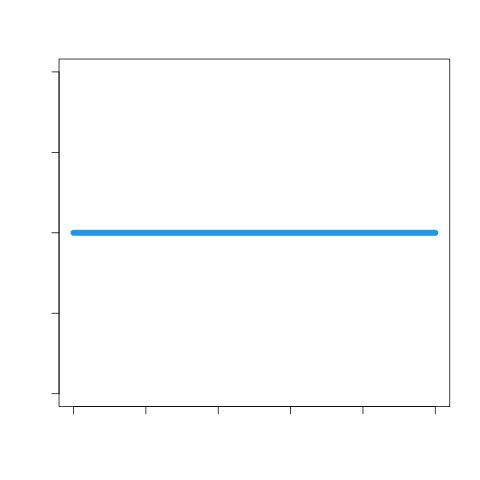
\includegraphics[width=.18\textwidth]{\fignet/FigMotifsBEDD-dist-h10} \end{tabular} &
    \begin{tabular}{c} 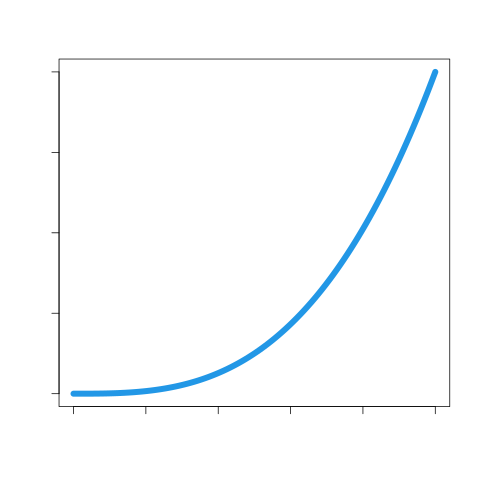
\includegraphics[width=.18\textwidth]{\fignet/FigMotifsBEDD-dist-h40} \end{tabular} \\
    \begin{tabular}{c} $g_0(u) =$ \end{tabular} &
    \begin{tabular}{c} 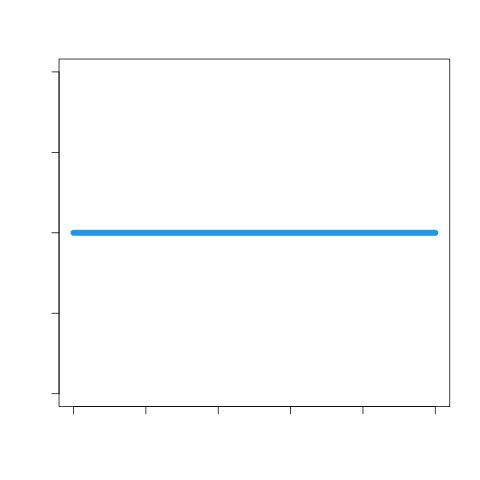
\includegraphics[width=.18\textwidth]{\fignet/FigMotifsBEDD-dist-g10} \end{tabular} &
    \begin{tabular}{c} 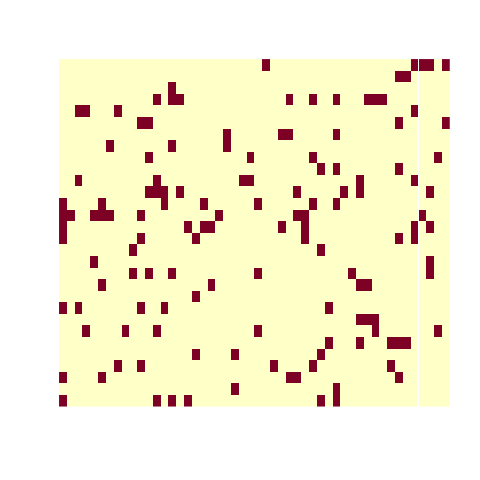
\includegraphics[width=.18\textwidth]{\fignet/FigMotifsBEDD-adj-g10-h10} \end{tabular} &
    \begin{tabular}{c} 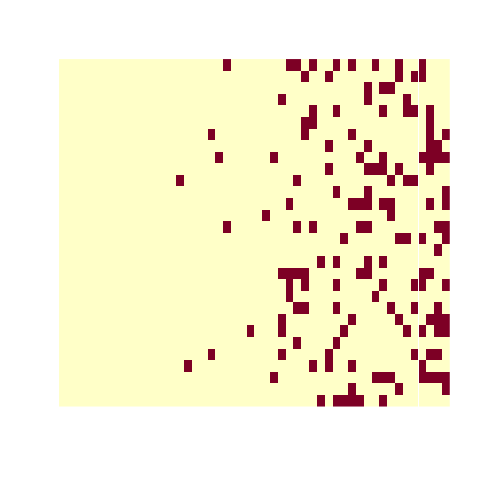
\includegraphics[width=.18\textwidth]{\fignet/FigMotifsBEDD-adj-g10-h40} \end{tabular} \\
    \begin{tabular}{c} $g(u) =$ \end{tabular} &
    \begin{tabular}{c} 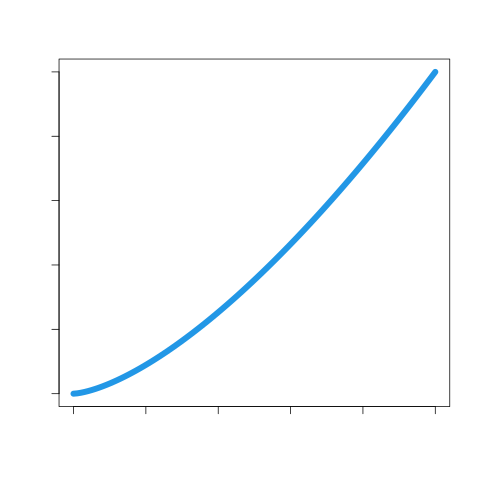
\includegraphics[width=.18\textwidth]{\fignet/FigMotifsBEDD-dist-g25} \end{tabular} &
    \begin{tabular}{c} 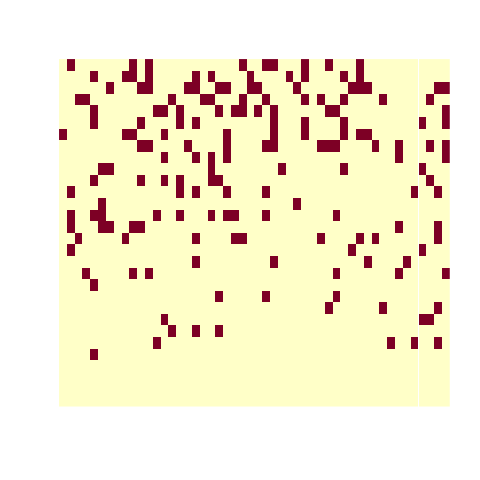
\includegraphics[width=.18\textwidth]{\fignet/FigMotifsBEDD-adj-g25-h10} \end{tabular} &
    \begin{tabular}{c} 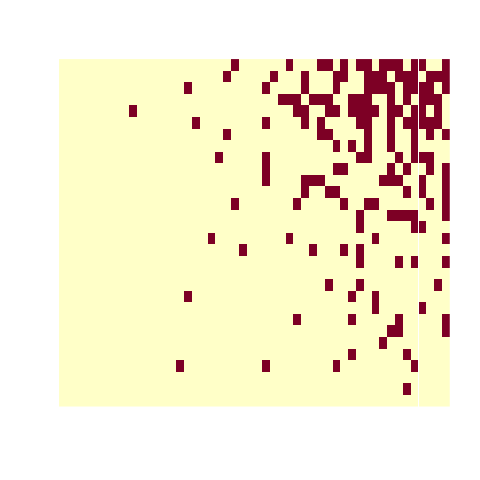
\includegraphics[width=.18\textwidth]{\fignet/FigMotifsBEDD-adj-g25-h40} \end{tabular} \\
  \end{tabular}
  
  \ra \emphase{Row-column exchangeable model} (species are 'exchangeable')
  
%   \bigskip 
%   \paragraph{Sufficient statistics} to fit BEDD: stars (top, bottom, single edge) frequencies

}

%==================================================================
\frame{ \frametitle{$U$-statistics}

  \begin{tabular}{ll}
    \hspace{-.04\textwidth}
    \begin{tabular}{p{.6\textwidth}}
      \paragraph{Kernel.} 
      For a quadruplet made of 2~plants $(i_1, i_2)$ $\times$ 2~insects $(j_1, j_2)$, define
      $$
      h(Y_{i_1, j_1}, Y_{i_1, j_2}, Y_{i_2, j_1}, Y_{i_2, j_2})
      $$
      
      \onslide+<2->{\bigskip \bigskip 
      \paragraph{$U$-statistic.} Mean over all quadruplets
      $$
      U = \binom{m}{2}^{-1} \binom{n}{2}^{-1} \sum_{i_1 ,i_2, j_1, j_2} h(Y_{i_1, j_1}, Y_{i_1, j_2}, Y_{i_2, j_1}, Y_{i_2, j_2})
      $$}

      \onslide+<3->{\bigskip \bigskip 
      \paragraph{Theory.} Many (old) results \refer{Hoe48} about the asymptotic distribution of $U$-statistics
      $$
      U \overset{\Lcal}{\longrightarrow} \Ncal(\mu, \sigma^2),
      $$
      ... but not for matrix quadruplets.}

    \end{tabular}
    &
    \hspace{-.2\textwidth}
    \begin{tabular}{p{.45\textwidth}}
      \onslide+<1->{
      \includegraphics[width=.6\textwidth]{\fignet/FigUstatsBEDD-ustat-f25-g40}
      }
    \end{tabular} 
  \end{tabular}

}

%==================================================================
\frame{ \frametitle{Tam's work}

  \paragraph{Theory.} 
  Under (some) row-exchangeable models, $U$-statistics based on matrix quadruplets are asymptotically normal. \refer{LeM21}
  
  \bigskip \bigskip 
  \paragraph{Application.} Under the bipartite expected degree distribution model, \\ ~
  \begin{itemize}
   \item \pause take
   $$
   h(Y_{i_1, j_1}, Y_{i_1, j_2}, Y_{i_2, j_1}, Y_{i_2, j_2}) = 
   \frac12 \left(Y_{i_1, j_1} Y_{i_1, j_2} + Y_{i_2, j_1} Y_{i_2, j_2} \right)
   $$
   \item \pause we have
   $$
   \Esp \left[h(Y_{i_1, j_1}, Y_{i_1, j_2}, Y_{i_2, j_1}, Y_{i_2, j_2})\right] = \lambda^2 \int f^2(u) \d u
   $$
   \item \pause where
   $$
   \left\{\int f^2(u) \d u = 1\right\}
   \quad \Leftrightarrow \quad \{f(u) \equiv 1\}
   \quad \Leftrightarrow \quad \{\text{no imbalance among plants}\}
   $$
   \item \pause so, possible to design a test for
   $$
   H_0 = \{\text{no imbalance among plants}\}
   $$
  \end{itemize}
  
  \bigskip
  \ra On-going PhD under the supervision of S. Donnet, F. Massol and S. Robin
  
}

%==================================================================
%==================================================================
\backupbegin
%==================================================================
\frame{ \frametitle{References}

  {\tiny
  \bibliography{/home/robin/Biblio/BibGene}
  \bibliographystyle{alpha}
  }
}

\backupend

%==================================================================
%==================================================================
\end{document}
%==================================================================
%==================================================================

\begin{tabular}{ll}
  \hspace{-.04\textwidth}
  \begin{tabular}{p{.45\textwidth}}
  \end{tabular}
  &
  \hspace{-.05\textwidth}
  \begin{tabular}{p{.45\textwidth}}
  \end{tabular} 
\end{tabular}

